\begin{refsection}

\chapter{Supplements to Chapter 3}\label{appendix:a3}




The ground states of the neutral and anionic clusters \ch{ScSi2^{-/0}} should be correctly determined. To do so, the optimization processes are performed with regard to many possible spins and isomers. The results of the optimization processes also help to cross out states whose relative energies are significantly higher than the lowest ones. After geometrically optimized at many possible spin multiplicities, the relative energies of the linear and cyclic isomers are collected and visualized in Figure \ref{a3fig:surface}. To be more detailed, a triplet state of the cyclic isomer is determined to be the most stable structure on the potential surface at the B3LYP and BP86 levels of theory, although the B3LYP calculations placed this state only 0.12 eV higher than the lowest one of the singlet states. Concerning the linear isomer, the most stable state of this anionic isomer is relatively located at 0.34 eV higher than the lowest triplet state. Therefore, the linear isomer of the anionic cluster can be safely neglected when finding the ground state of the anionic cluster \ch{ScSi2-}. As for the neutral cluster, both B3LYP and BP86 consistently estimated a doublet state as the most stable state. Energies of all the states of the linear isomer are significantly higher than those of the cyclic corresponding states, and especially much higher than the lowest one of a doublet state. Particularly, the most stable state of the neutral cyclic isomer, a doublet state, is around 1.50 eV more stable than that of the neutral linear isomer at both B3LYP and BP86 calculations. Therefore, the anionic and neutral cyclic isomers are used for further calculations to locate the ground states and low-lying states involving in ionization processes. Also, all the septet, sextet and octet states of these isomers would be no longer considered, since their relative energies are far higher than the lowest one of the triplet states.




\begin{figure}[htb!]
	\centering
	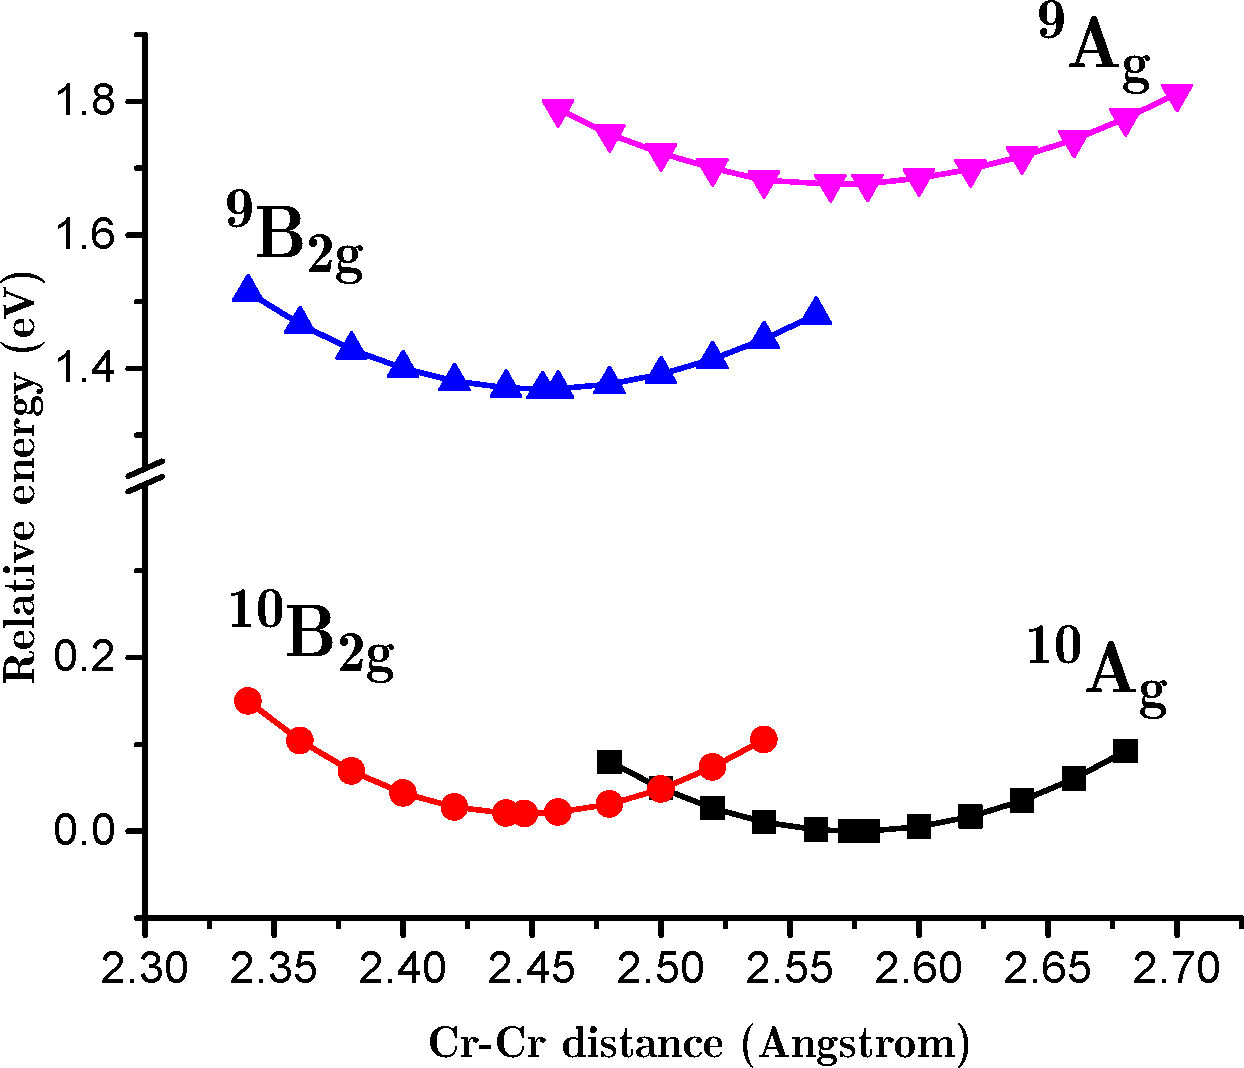
\includegraphics[width=\textwidth]{potential-surface}
	\caption{Potential surfaces of the linear and cyclic structures of \ch{ScSi2^{-/0}} at the B3LYP (on the left-hand side) and BP86 (on the right-hand side) levels of theory. Relative energies of the cyclic and liner isomers are noted as blue squares and red circles, respectively.}
	\label{a3fig:surface}
\end{figure}




Both singlet and a triplet states of the cyclic isomer are found to be more stable than other spin states. Therefore, to roughly estimate the adiabatic energy barrier for the interconversion between the linear and cyclic isomers, we calculated the total energies of both states when their geometries change from the linear form to the cyclic one (cf. Figure \ref{fig3:scsi2} for both geometrical forms). The energy profiles of both spin states are depicted in Figure \ref{a3fig:crossing} using (U)B3LYP computations. In both states, the linear form is only a very shallow minimum on the potential energy surface. They are not expected to be stable.



\begin{figure}[htb!]
	\centering
	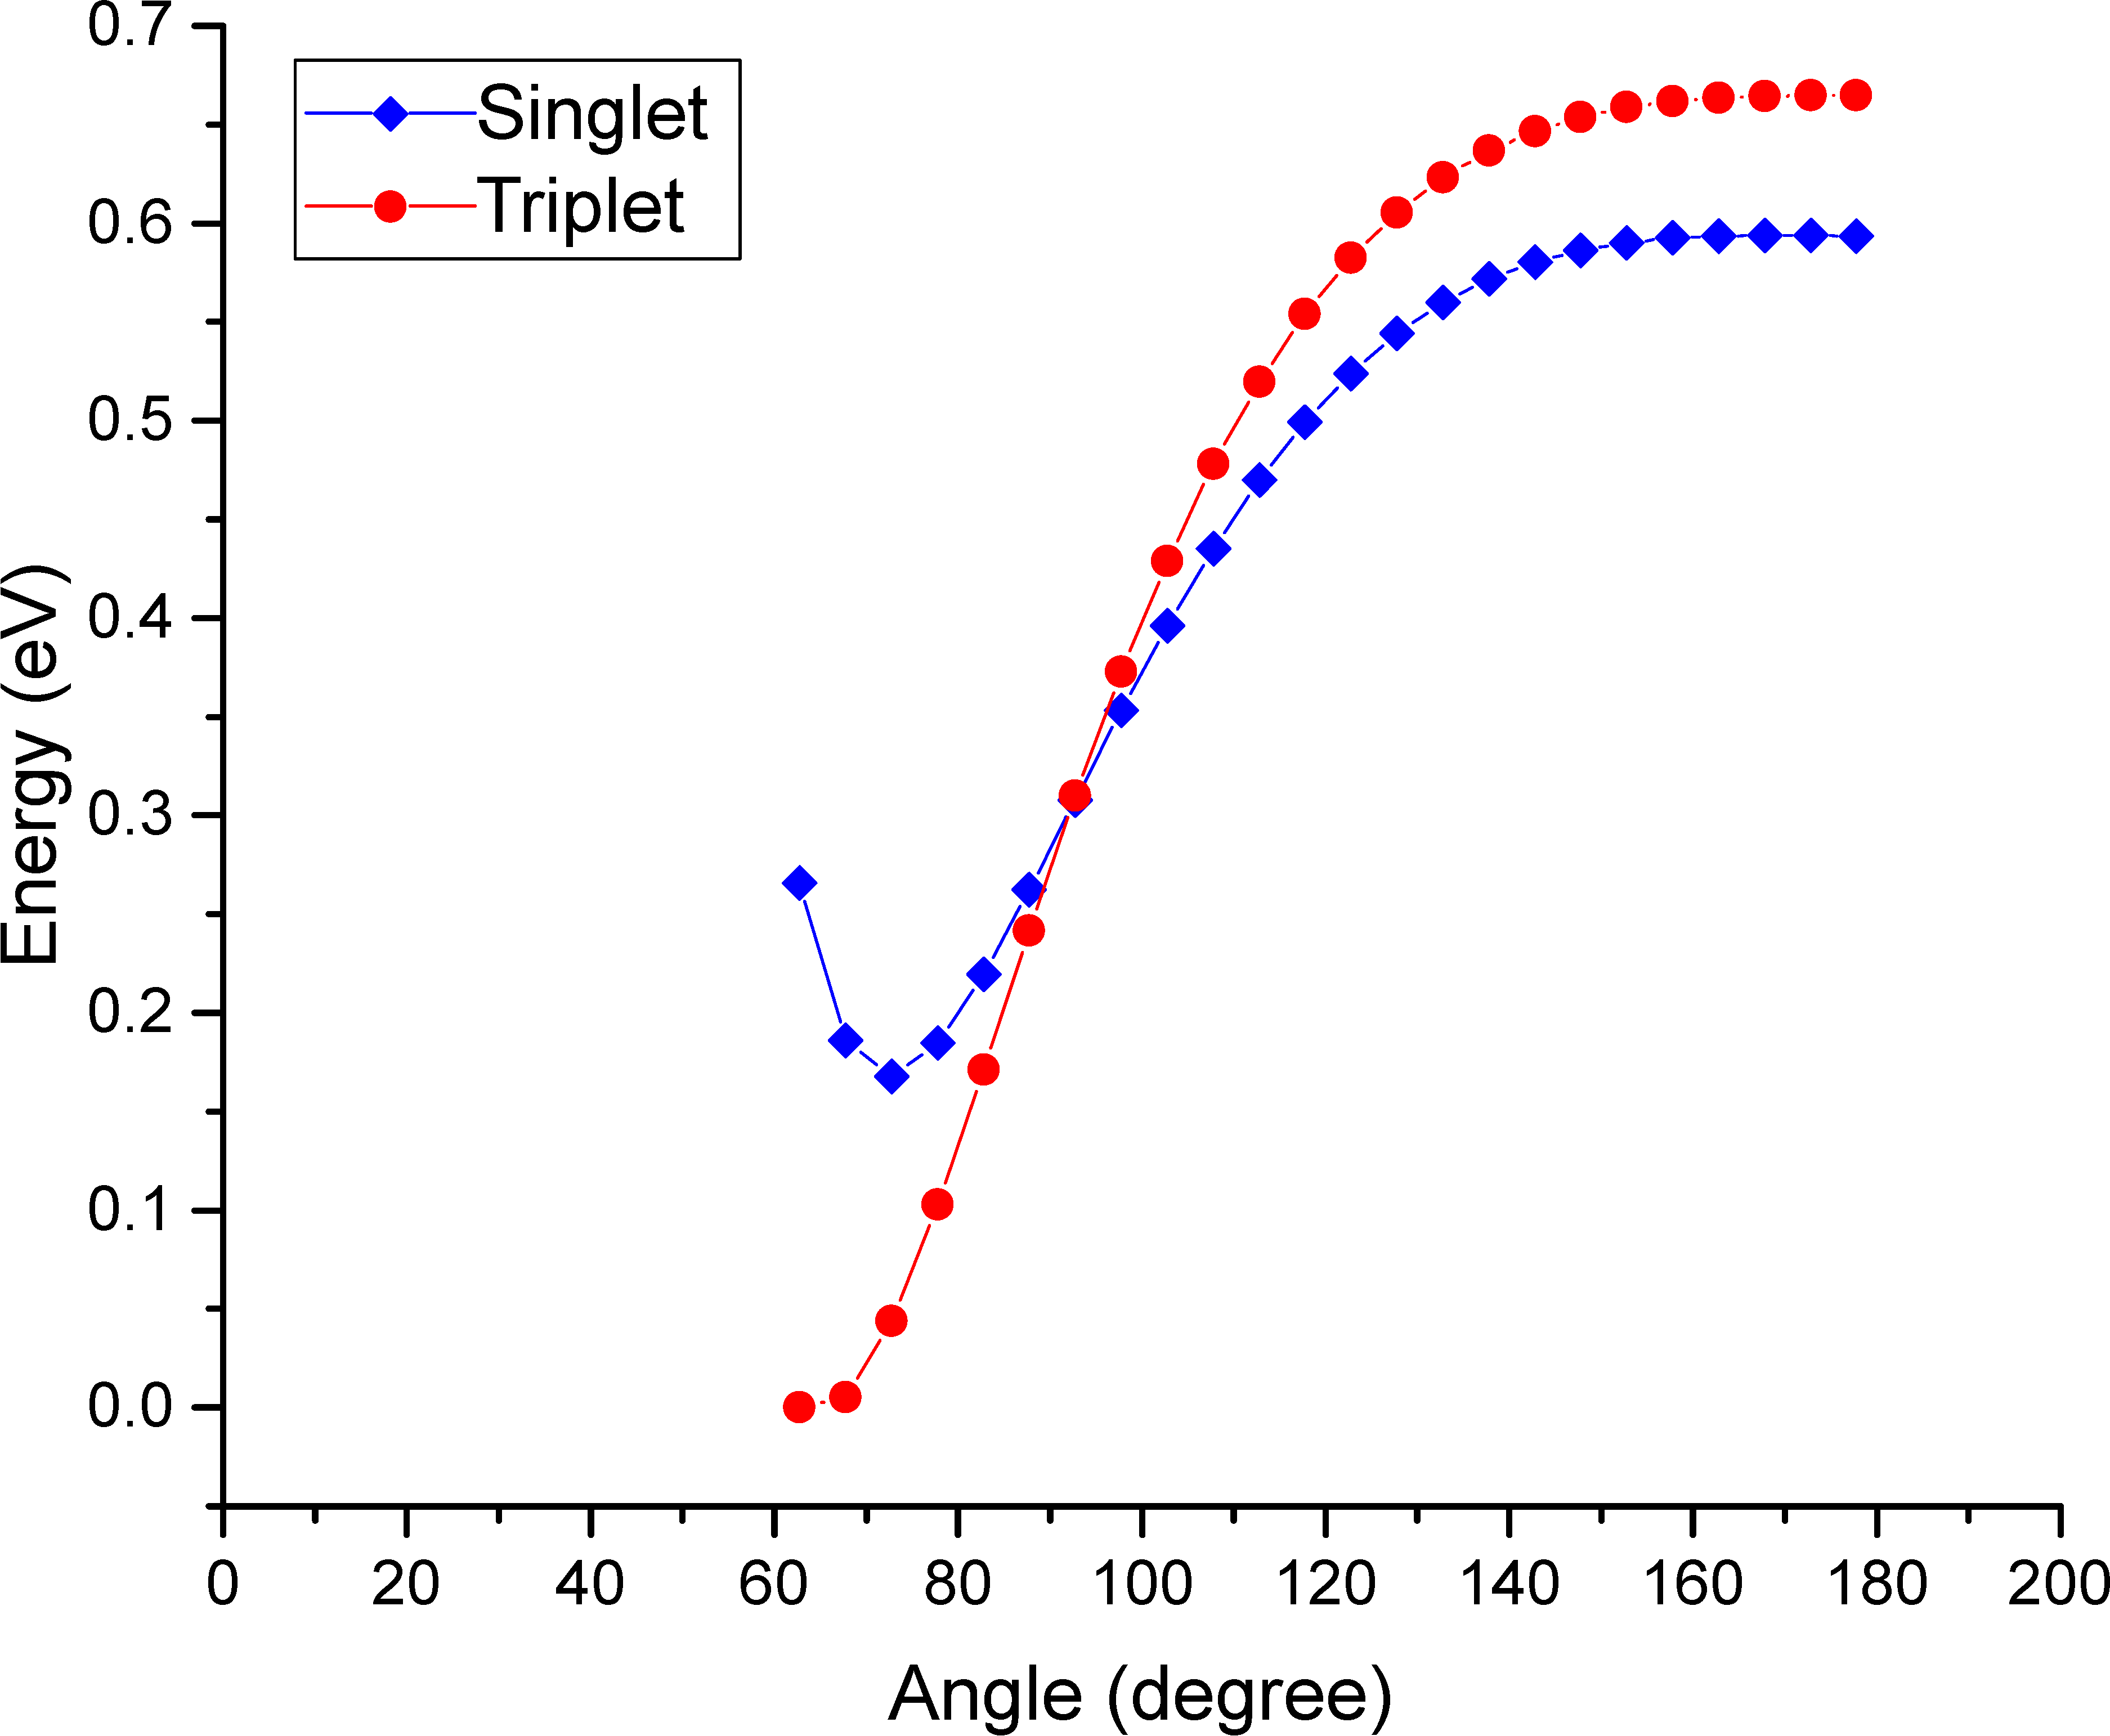
\includegraphics[width=0.7\textwidth]{spin-state-crossing.pdf}
	\caption{Adiabatic energy profiles of the singlet and the triplet state changing from the cyclic structure to the linear one. An adiabatic crossing transition between two states can be found at around 0.30 eV (without \acrshort{zpe} correction). All the optimized energies are calculated at the B3LYP/aug-cc-PVTZ level of theory.}
	\label{a3fig:crossing}
\end{figure}





Figure \ref{a3fig:crossing} points out a crossing between both states at a bond angle of $\sim$90 degree, being around 0.30 eV above the cyclic form. The energy profiles also suggest a possible inter-crossing mechanism with respect to geometrical changes from the cyclic isomer to another cyclic form but in another spin state. A change from the cyclic triplet state goes through the crossing point (at 90 degree at 0.30 eV) and then follows the energy profile of the singlet state giving the cyclic form.




To ensure the linear isomer is substantially less stable than the cyclic one, all states of singlet and triplet are optimized at the \acrshort{caspt2} level of theory, since from the previous calculation step, we found that a singlet and a triplet state of the linear isomer are lower than other spin-multiplicity states within this linear isomer. In Table \ref{a3tbl:RElinear}, the relative energies of all singlet and triplet states of the anionic linear isomer are given. These relative energies to the anionic ground state $^3$B$_2$, a state of the cyclic isomer, are calculated at \acrshort{caspt2} levels of theory only because in part many singlet states cannot obtained at single-reference theories (\acrshort{dft} and \acrshort{rccsd}(T)). These values apparently prove that the lowest state of the anionic linear isomer $^1$A$_1$, which is 0.66 eV higher than the anionic cyclic isomer, is significant higher than the global anionic ground state $^3$B$_2$. Again, we can confidently cross out the anionic linear isomer as the starting geometrical structure from which the photodetachments occur. And therefore, all states of the linear isomer are not being considered in assignments of the anion photoelectron bands.




\begin{table}[htbp!]
    \centering
    \begin{threeparttable}
    \caption{Relative energies of the anionic linear isomer’s states optimized at \acrshort{caspt2} levels of theory. Only low-lying states of singlet and triplet are tabulated}
    \label{a3tbl:RElinear}
    \begin{tabular}{@{}lllcccc@{}}
    \toprule
    \multirow{3}{*}{cluster}       & \multirow{3}{*}{state} &  & \multicolumn{2}{c}{\acrshort{caspt2} Geometry (\AA)} & \multirow{3}{*}{\begin{tabular}[c]{@{}c@{}}symmetric \\ vibrational\\  frequency (cm$^{-1}$)\tnote{(a)}\end{tabular}} & \multirow{3}{*}{\begin{tabular}[c]{@{}c@{}}\acrshort{caspt2} \\ relative \\ energy (eV)\end{tabular}} \\ \cmidrule(lr){4-5}
    &      &  & \multirow{2}{*}{\ch{Sc-Si}}      &  \multirow{2}{*}{\ch{Si-Si}}     &            &           \\   
    &      &  &  &  &            &           \\ \cmidrule(r){1-2} \cmidrule(l){4-7} 
    \multirow{8}{*}{\begin{tabular}[c]{@{}l@{}}linear \\ \ch{ScSi2-}\end{tabular}} & 1A1  &  & 2.46 & 2.13  & 308, 637 & 0.66  \\
    & $^1$B$_1$  &  & 2.57  & 2.14  & 247, 599   & 1.63      \\
    & $^1$B$_2$  &  & 2.57  & 2.14  & 250, 617   & 1.63      \\
    & $^1$A$_2$  &  & 2.95  & 2.16  & 139, 590   & 1.93      \\
    & $^3$A$_1$  &  & 2.54  & 2.13  & 266, 618   & 1.24      \\
    & $^3$B$_1$  &  & 2.57  & 2.13  & 259, 618   & 1.24      \\
    & $^3$B$_2$  &  & 2.57  & 2.13  & 258, 618   & 1.24      \\
    & $^3$A$_2$  &  & 2.92  & 2.16  & 146, 578   & 1.81      \\ \bottomrule
    \end{tabular}
    \begin{tablenotes}
        \item[(a)] The analysis of vibrations are done with regards to C$_{2v}$ symmetry, which results in obtaining totally symmetric modes of vibrations only.
    \end{tablenotes}
    \end{threeparttable}
    \end{table}




In Table \ref{a3tbl:ZPE}, we provide relative energies of many neutral states to the anionic ground state of the cyclic isomer and the \acrshort{zpe}s calculated at B3LYP level of theory. Apparently, the values of \acrshort{zpe} are very small, around 0.06 eV, compared to the absolute values of electronic energies. As seen in Table \ref{a3tbl:ZPE}, zero-point energies do not significantly affect the relative positions of states on the potential hypersurface at the B3LYP level of theory. This fact is mentioned elsewhere \cite{a3:1} when studying electronic structures of ground states and low-lying states of many clusters, and the ZPE correction was, therefore, safely ignored in several related publications. \cite{a3:2, a3:3, a3:4, a3:5, a3:6} Hence, all the relative energies in this work are pure electronic energies without \acrshort{zpe}s.




\begin{table}[htbp!]
    \centering
    \caption{The relative energies of accessible states at the B3LYP level energy without and with corrected zero-point energy. The \acrshort{zpe}s are calculated with the triple-$\zeta$ basis set aug-cc-pVTZ-DK by performing vibrational calculations}
    \label{a3tbl:ZPE}
    \begin{tabular}{@{}lcccc@{}}
    \toprule
    cluster       & state & \begin{tabular}[c]{@{}c@{}}relative energy \\ without corrected \\ \acrshort{zpe} (eV)\end{tabular} & \acrshort{zpe} (eV) & \begin{tabular}[c]{@{}c@{}}relative energy \\ with corrected \\ \acrshort{zpe} (eV)\end{tabular} \\ \midrule
    cyclic \ch{ScSi2-}   & $^3$A$_1$   & 0.45  & 0.057    & 0.44  \\
                         & $^3$B$_1$   & 0.59  & 0.060    & 0.60  \\
                         & $^3$B$_2$   & 0.00  & 0.061    & 0.00  \\
                         & $^3$A$_2$   & 0.31  & 0.058    & 0.31  \\
    cyclic \ch{ScSi2^0}  & $^2$A$_1$   & 1.61  & 0.066    & 1.61  \\
                         & $^2$B$_1$   & 2.10  & 0.061    & 2.09  \\
                         & $^2$B$_2$   & 1.34  & 0.063    & 1.33  \\
                         & $^2$A$_2$   & 1.65  & 0.063    & 1.65  \\
                         & $^4$A$_1$   & 2.50  & 0.054    & 2.50  \\
                         & $^4$B$_1$   & 2.53  & 0.060    & 2.53  \\
                         & $^4$B$_2$   & 2.29  & 0.061    & 2.29  \\
                         & $^4$A$_2$   & 2.36  & 0.055    & 2.35  \\ \bottomrule
    \end{tabular}
    \end{table}






















%\instructionsappendices


%%%%%%%%%%%%%%%%%%%%%%%%%%%%%%%%%%%%%%%%%%%%%%%%%%
% Keep the following \cleardoublepage at the end of this file, 
% otherwise \includeonly includes empty pages.
%\cleardoublepage

% vim: tw=70 nocindent expandtab foldmethod=marker foldmarker={{{}{,}{}}}



\cleardoublepage

\includebibliography
\printbibliography[heading=subbibliography] % print section bibliography

\end{refsection}